\subsection{Problem formulation}
\label{sec:problem_formulation}
In this section, the problem of Learning from Demonstration, also known as Imitation Learning (IL), will be formalized.

The core idea behind IL is to program a robot by allowing a human expert to demonstrate how to solve a specific task. This approach avoids methods that demand intricate, handcrafted rules dictating the actions of machines and the dynamics of their operating environments, which require significant time and coding expertise. To achieve this goal, a way to transfer knowledge from the expert to the robot is necessary. One possibility is to leverage \textit{data-driven} methods that can extrapolate control rules from demonstrated trajectories~\cite{osa2018algorithmic}.

In this context, we need to define two general actors: the \textbf{expert}, who demonstrates the desired behaviors, and the \textbf{learner}, whose goal is to learn and replicate the behaviors demonstrated by the expert~\cite{osa2018algorithmic,zare2024survey}. Both the expert behaviors and the learner behaviors are described in terms of \textbf{policy}, generally denoted as $\pi^{E}$ and $\pi^{L}$ respectively.

Since IL relies on expert demonstrations, these are collected in a dataset $\mathcal{D}^{E}=\left\{\left(\boldsymbol{\tau}^{E}_{i}, c_{i}\right)\right\}_{i=1}^{N}$, where:
\begin{itemize}[noitemsep]
    \item $\boldsymbol{\tau}^{E}_{i}$ is the $i^{th}$ demonstrated trajectory, generated by the expert policy $\pi^{E}\sim\boldsymbol{\tau}^{E}_{i}$. It can be described as:
        \begin{itemize}[noitemsep]
            \item A \textit{state-action sequence}, i.e., $\boldsymbol{\tau}_{i} = [s_{0}, a_{0}, \dots, s_{T}, a_{T}]$, when the ground truth action performed by the expert is available.
            \item A \textit{state-only sequence}, i.e., $\boldsymbol{\tau}_{i} = [s_{0}, \dots, s_{T}]$, when the ground truth action is not available.
        \end{itemize}
    \item $c_{i}$ is the \textit{context-vector}, containing task-related information such as the initial state of the system $s_{0}$, the position of the target object, or a representation of the task to be executed (e.g., a natural language description of the task or video demonstrations).
\end{itemize}

The state $s_{t}$ can be defined in various ways. RGB images have been used in different works, either from a third-person point of view \cite{james2018task_embedded}, representing the robot and its workspace, or from a first-person point of view with the camera mounted on the robot \cite{jang2022bc_z} or the gripper \cite{mees2022calvin}. Additionally, 3D point-clouds generated by RGB-D images can also be used \cite{shridhar2023perceiver}. This high-level state representation can be enriched with proprioceptive signals such as joint positions, velocities, and torques \cite{zhang2018deep_vr_teleoperation}.

Regarding the policy, the predicted action, $\hat{a}_{t}$, can be generated into two distinct ways. In one case, it is described as a \textit{deterministic function}, meaning that it directly determines the action as follows: $\hat{a}_{t} = \pi^{L}(s_{t}, c_{i})$\cite{jang2022bc_z}. In the other case, it takes on a probabilistic definition, where it represents a probability distribution from which to sample the desired action: $\hat{a}_{t} \sim \pi^{L}(s_{t}, c_{i})$~\cite{mandi2022towards_more_generalizable_one_shot}.

According to the definitions given in~\cite{osa2018algorithmic,fang2019survey}, the learner policy $\pi^{L}$ can be defined with respect to different abstraction levels:
\begin{itemize}
    \item \textit{Symbolic Characterization}, the policy maps states, and context to a sequence of options, i.e., $\pi: s_{t}, c \rightarrow [o_1, \dots, o_T]$, where each option is a sequence of actions. With this representation, complex tasks can be decomposed into a sequence of simple movements. However, it is hard to achieve an accurate task segmentation and motion ordering;
    \item \textit{Trajectory Characterization}, the policy maps context to trajectory, i.e., $\pi: c \rightarrow \boldsymbol{\tau}$. Because it allows the initial state to be mapped to a complete sequence of actions, this representation can be used to obtain the options in the Symbolic Representation. However, they need as many dynamic features as possible, that can be difficult to obtain;
    \item \textit{State-Action Characterization}, the policy maps states(-context) to actions, i.e., $\pi: s_{t}, c \rightarrow a_{t}$. This representation makes it possible to map the current state directly to the corresponding action. However, it is easy for errors to accumulate in long-term processes. The action $a_{t}$ can also be defined in various ways, depending on the type of control implemented by the method. Some methods operate in the joint-space, predicting motor control signals such as positions, velocities, and torques~\cite{zhang2018deep_vr_teleoperation}. Other methods work in the operational space, where actions are assigned either an absolute pose with respect to a world frame $\mathcal{W}$, i.e., $a_{i} = \left[p_x^{\mathcal{W}}, p_y^{\mathcal{W}}, p_z^{\mathcal{W}}, r_x^{\mathcal{W}}, r_y^{\mathcal{W}}, r_z^{\mathcal{W}}\right]$~\cite{mandi2022towards_more_generalizable_one_shot}, or a displacement relative to the current gripper position, i.e., $a_{i} = \left[\Delta p_x^{\mathcal{W}}, \Delta p_y^{\mathcal{W}}, \Delta p_z^{\mathcal{W}}, \Delta r_x^{\mathcal{W}}, \Delta r_y^{\mathcal{W}}, \Delta r_z^{\mathcal{W}}\right]$~\cite{jang2022bc_z}.

\end{itemize}

The expert and the learner, through their policies $\pi^{E}$ and $\pi^{L}$, act on an environment modeled as a \textit{Markov Decision Process} (MDP)~\cite{kroemer2021review_robot_learning}. An MDP is defined as a tuple $(S, A, R, T, \gamma)$, where:
\begin{itemize}
    \item $S \subseteq \mathbb{R}^{n}$ is the set of states (e.g., joint positions and/or images).
    \item $A \subseteq \mathbb{R}^{n}$ is the set of actions (e.g., desired end-effector pose, desired joint torques).
    \item $R(s, a, s')$ is the \textit{reward function}, which expresses the immediate reward for executing action $a$ in state $s$ and transitioning to state $s'$.
    \item $T(s' | s, a)$ is the \textit{transition function}, which defines the probability of reaching state $s'$ after executing action $a$ in state $s$. This distribution, which describes the \textit{system dynamics}, can be given a priori or learned (Model-Based methods), or it may not be considered at all (Model-Free methods).
    \item $\gamma \in [0,1]$ is the discount factor, expressing the agent's preference for immediate rewards over future rewards.
\end{itemize}

With respect to the given MDP definition, the reward function plays different roles depending on the approach used:
\begin{itemize}
    \item In \textit{Behavioral Cloning} (BC) methods, the reward function is not explicitly used. Instead, a surrogate loss function is employed.
    \item In \textit{Inverse Reinforcement Learning} (IRL), the reward function is learned, under the assumption that the expert acts (near-)optimally with respect to some unknown reward function.
    \item In \textit{Generative Adversarial Imitation Learning} (GAIL) and \textit{Learning from Observations} (LfO), the role of the reward function varies based on the specific method, as will be explained in Section \textcolor{red}{TODO}.
\end{itemize}



\subsection{Source of demonstration}
\input{}
As stated in Section \ref{sec:problem_formulation}, IL methods rely on a dataset $\mathcal{D}^{E}$ of expert demonstrations. In this section, we will review the different ways to obtain these demonstrations, following the taxonomy proposed in \cite{fang2019survey}.
\begin{figure}[tb]
     \centering
     \begin{subfigure}[b]{0.45\textwidth}
         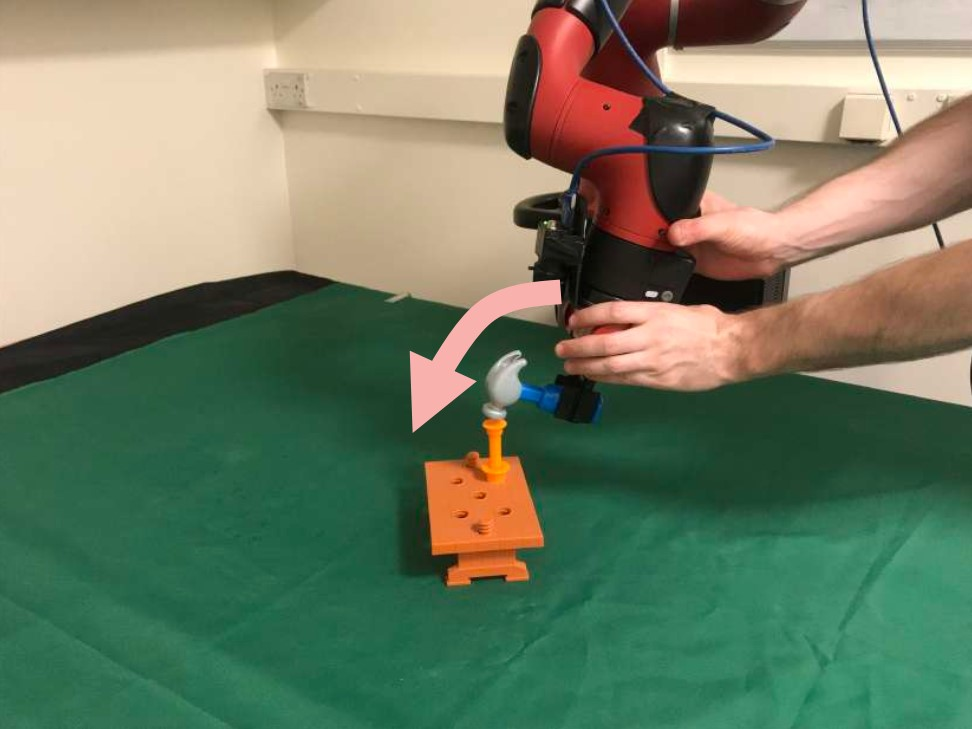
\includegraphics[width=\textwidth]{figures/images/direct_demonstration/kinesthetic.jpg}
         \caption{Example of kinesthetic teaching~\cite{johns2021coarse_to_fine}.}
         \label{fig:kinesthetic}
     \end{subfigure}
     \hfill
     \begin{subfigure}[b]{0.5\textwidth}
         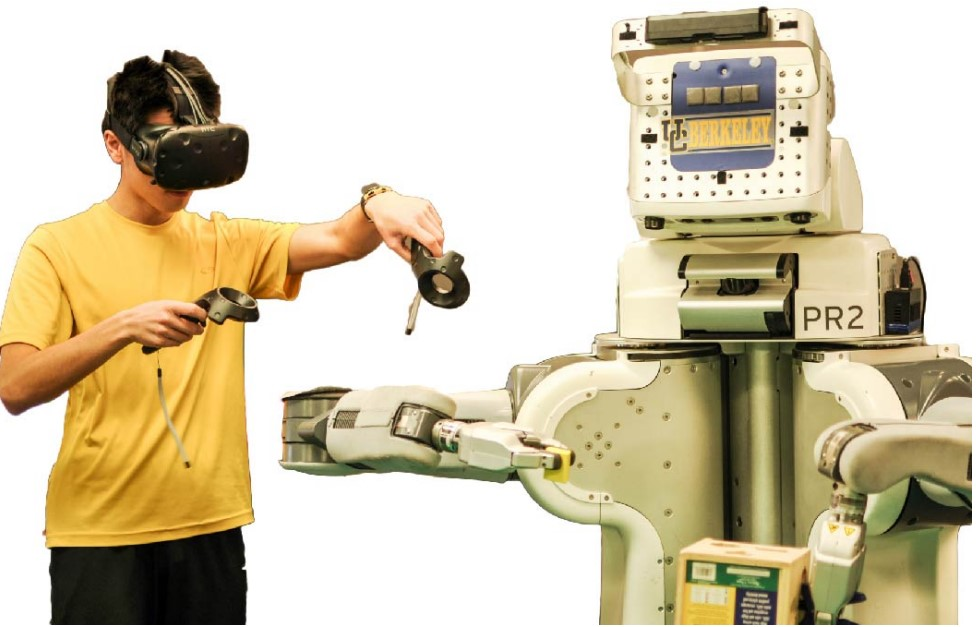
\includegraphics[width=\textwidth]{figures/images/direct_demonstration/teleoperation.jpg}
         \caption{Example of teleoperation~\cite{zhang2018deep_vr_teleoperation}.}
         \vspace{0.46cm}
         \label{fig:teleoperation}
     \end{subfigure}

    \caption{Examples of direct demonstration}
    \label{fig:direct_demonstrations}
\end{figure}


\paragraph*{Direct Demonstration}  \mbox{} \\
In the case of \textit{Direct Demonstration}, the expert trajectory is a state-action sequence, where the action is obtained directly from the robot. Specifically, the robot can be guided in task execution through \textit{kinesthetic teaching} \cite{caccavale2019kinesthetic,johns2021coarse_to_fine}, \textit{teleoperation} \cite{zhang2018deep_vr_teleoperation,mandlekar2018roboturk,jang2022bc_z,brohan2022rt,ebert22Bridge,mandlekar2023mimicgen}, or a \textit{(hand-)written policy} \cite{dasari2020robonet,dasari2021transformers_one_shot,mandi2022towards_more_generalizable_one_shot,chang2023one}.

In kinesthetic teaching (Figure \ref{fig:kinesthetic}), the human operator contacts and guides the robot, recording parameters such as the gripper pose, joint positions, and velocities. This has been one of the first approaches for the LfD problem \cite{lee2011incremental,saveriano2015incremental} because there is no need to consider differences in kinematics between human and robot. As a result, the data has less noise, and there is no need for expensive external tools for teleoperation. However, the robot must be passively controllable and require direct contact, which introduces safety problems and can be unintuitive for robots with multiple degrees of freedom.

In teleoperation (Figure \ref{fig:teleoperation}), the human operator remotely guides the robot with a joystick, control panel, or wearable device. These tools allow for higher safety since there is no direct contact between the robot and the human expert. Teleoperation systems have been used in various works. For example, the authors in \cite{mandlekar2018roboturk,mandlekar2019scaling} proposed a teleoperation framework named Roboturk, which enables the collection of large-scale demonstration datasets \cite{mandlekar2019scaling,mandlekar2022matters} for both simulated and real-world robots using a mobile phone as the controller. The authors in \cite{zhang2018deep_vr_teleoperation,jang2022bc_z,brohan2022rt} used virtual reality controllers, allowing the human operator to intuitively move in the 3D environment, mapping the pose of the controllers to the corresponding gripper pose. This technology is of interest because it provides a safe and intuitive way to teleoperate a robot. However, the main drawback is the lack of haptic feedback, which can be mitigated by using haptic interfaces such as \cite{cyberglove,touch}.

Demonstrations collected with hand-written policies rely on the fact that the expert has access to ground truth information, such as the position of the object of interest. This assumption can be valid when a simulated environment is used to train, test, and validate the proposed methods, as seen in \cite{dasari2021transformers_one_shot,mandi2022towards_more_generalizable_one_shot,chang2023one}. In these cases, the authors used a well-known simulation environment in the robotic learning community named Robosuite \cite{zhu2020robosuite}. Here, demonstrations were collected to train methods using hand-written policies that have access to ground truth positional information about the object of interest, solving tasks such as Pick-Place, Nut-Assembly, Stack-Block, and more. Simulation environments facilitate the evaluation of the proposed methods and ensure reproducibility and consistent testing. The idea of using hand-engineered policies is not limited to simulation environments. Indeed, the authors in \cite{dasari2020robonet} used automatic grasping primitives combined with diagonal Gaussian distributions to collect demonstrations on a real-world robot. This approach aims to collect as many trajectories as possible with minimal human effort.

\begin{figure}[tb]
     \centering
     \begin{subfigure}[b]{0.63\textwidth}
         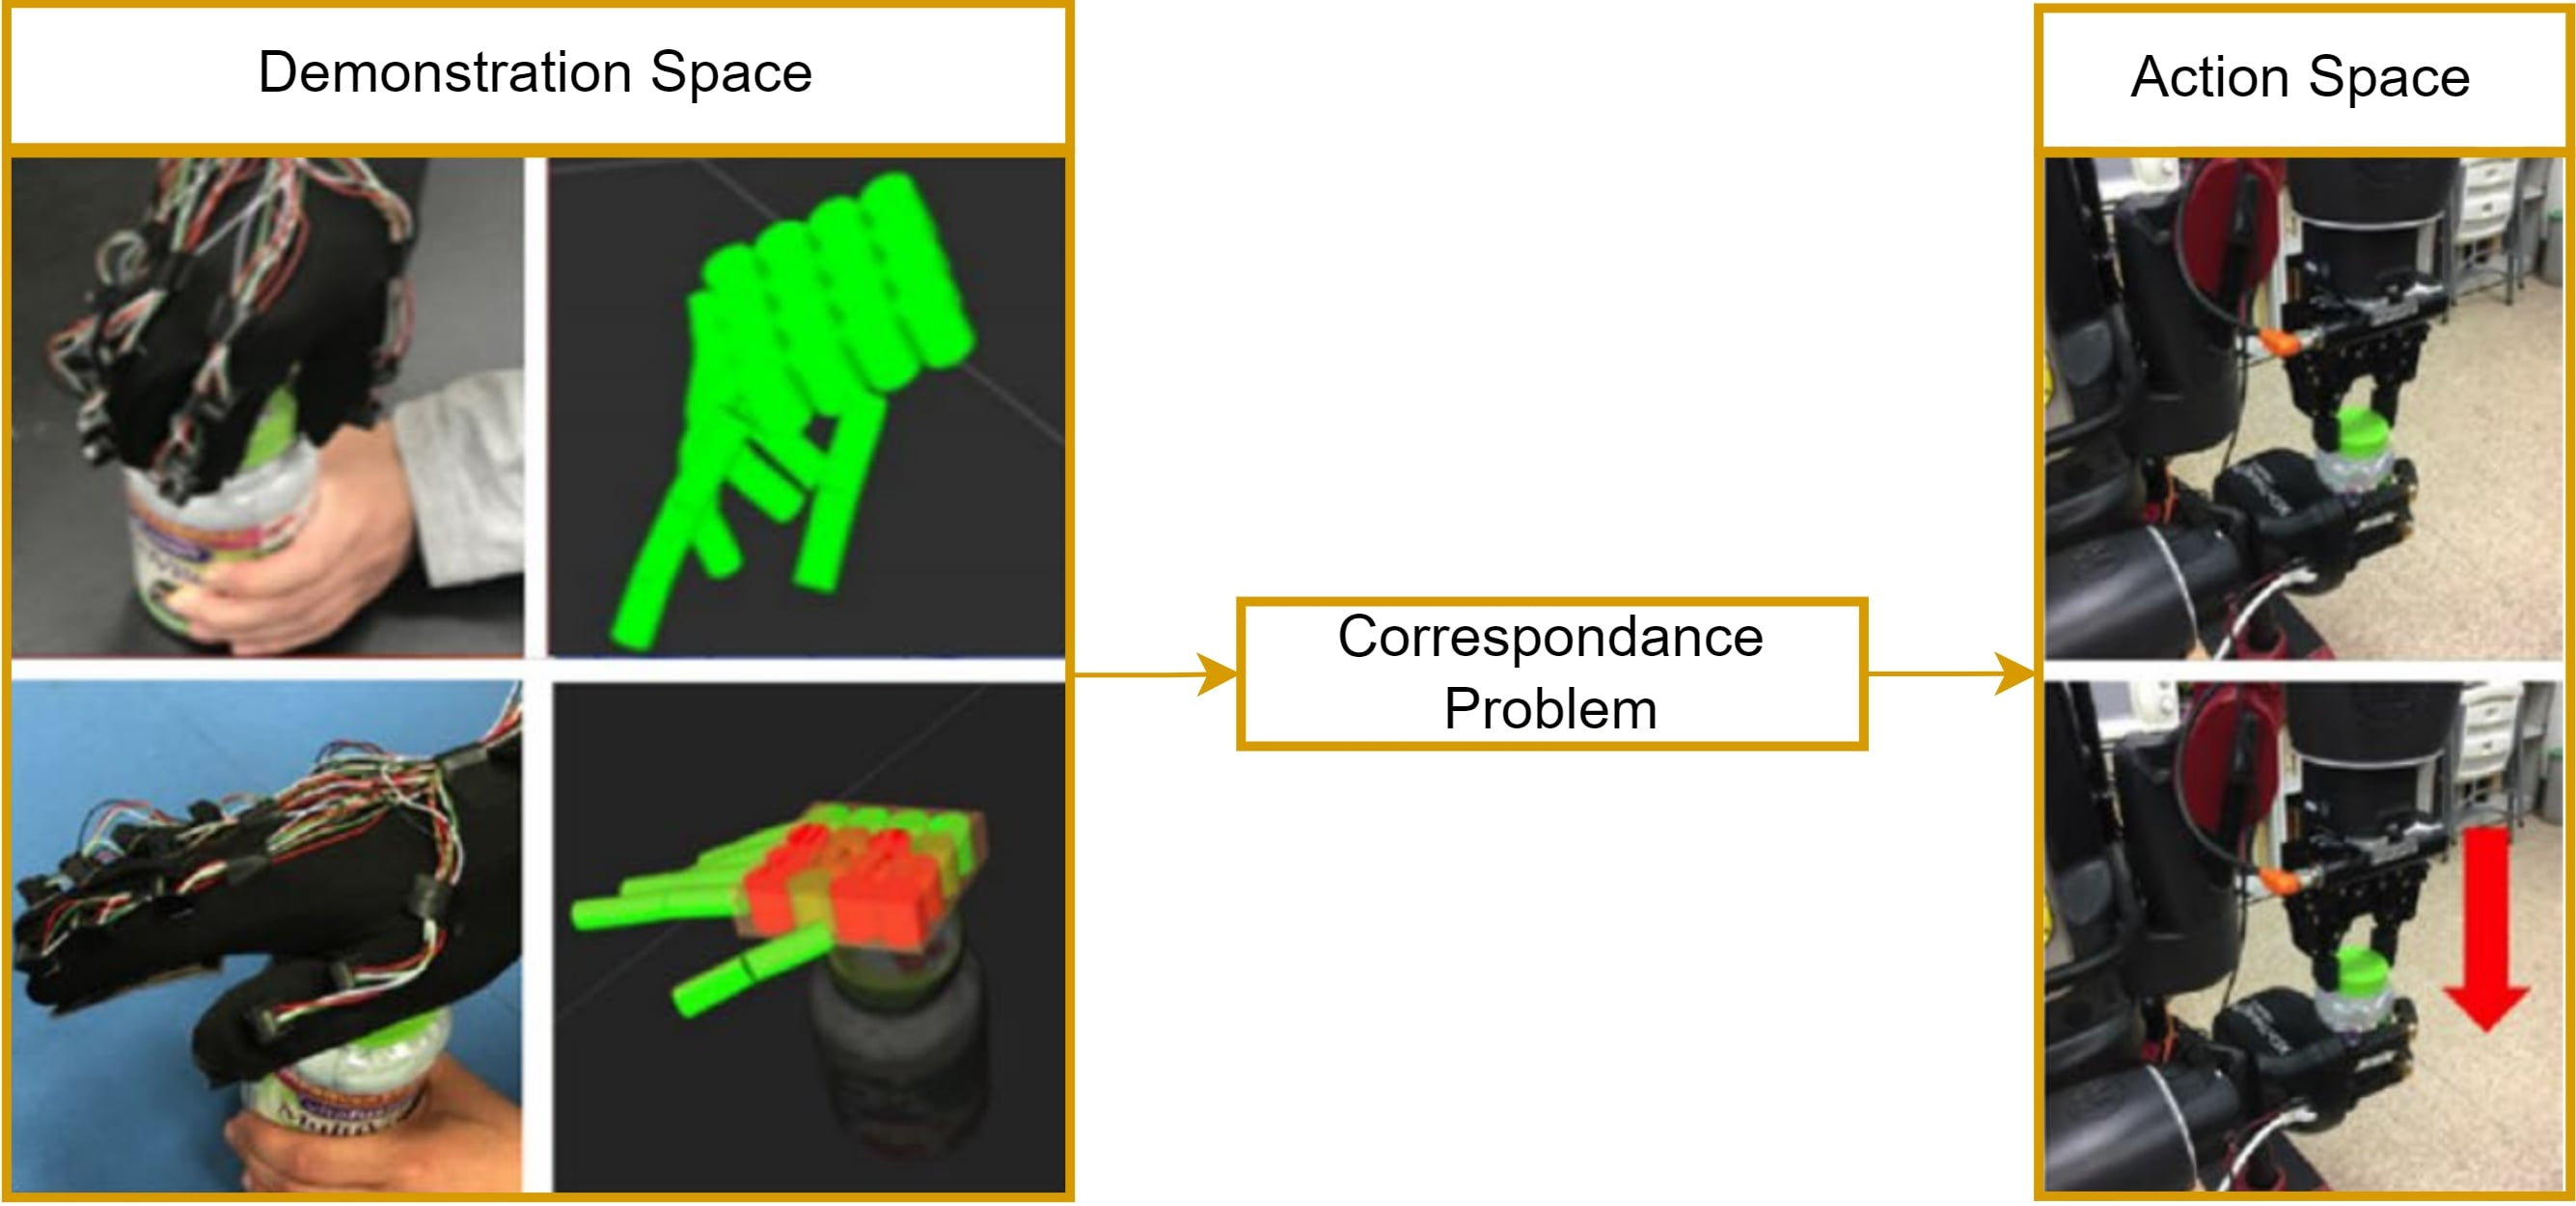
\includegraphics[width=\textwidth]{figures/images/wearable_indirect_teaching.jpg}
         \caption{Example of indirect demonstration based on wearable device~\cite{liu2019_mirroring_without_overimitation}.}
         \label{fig:wearable_indirect}
     \end{subfigure}
     \vfill
     \vfill
     \begin{subfigure}[b]{0.63\textwidth}
         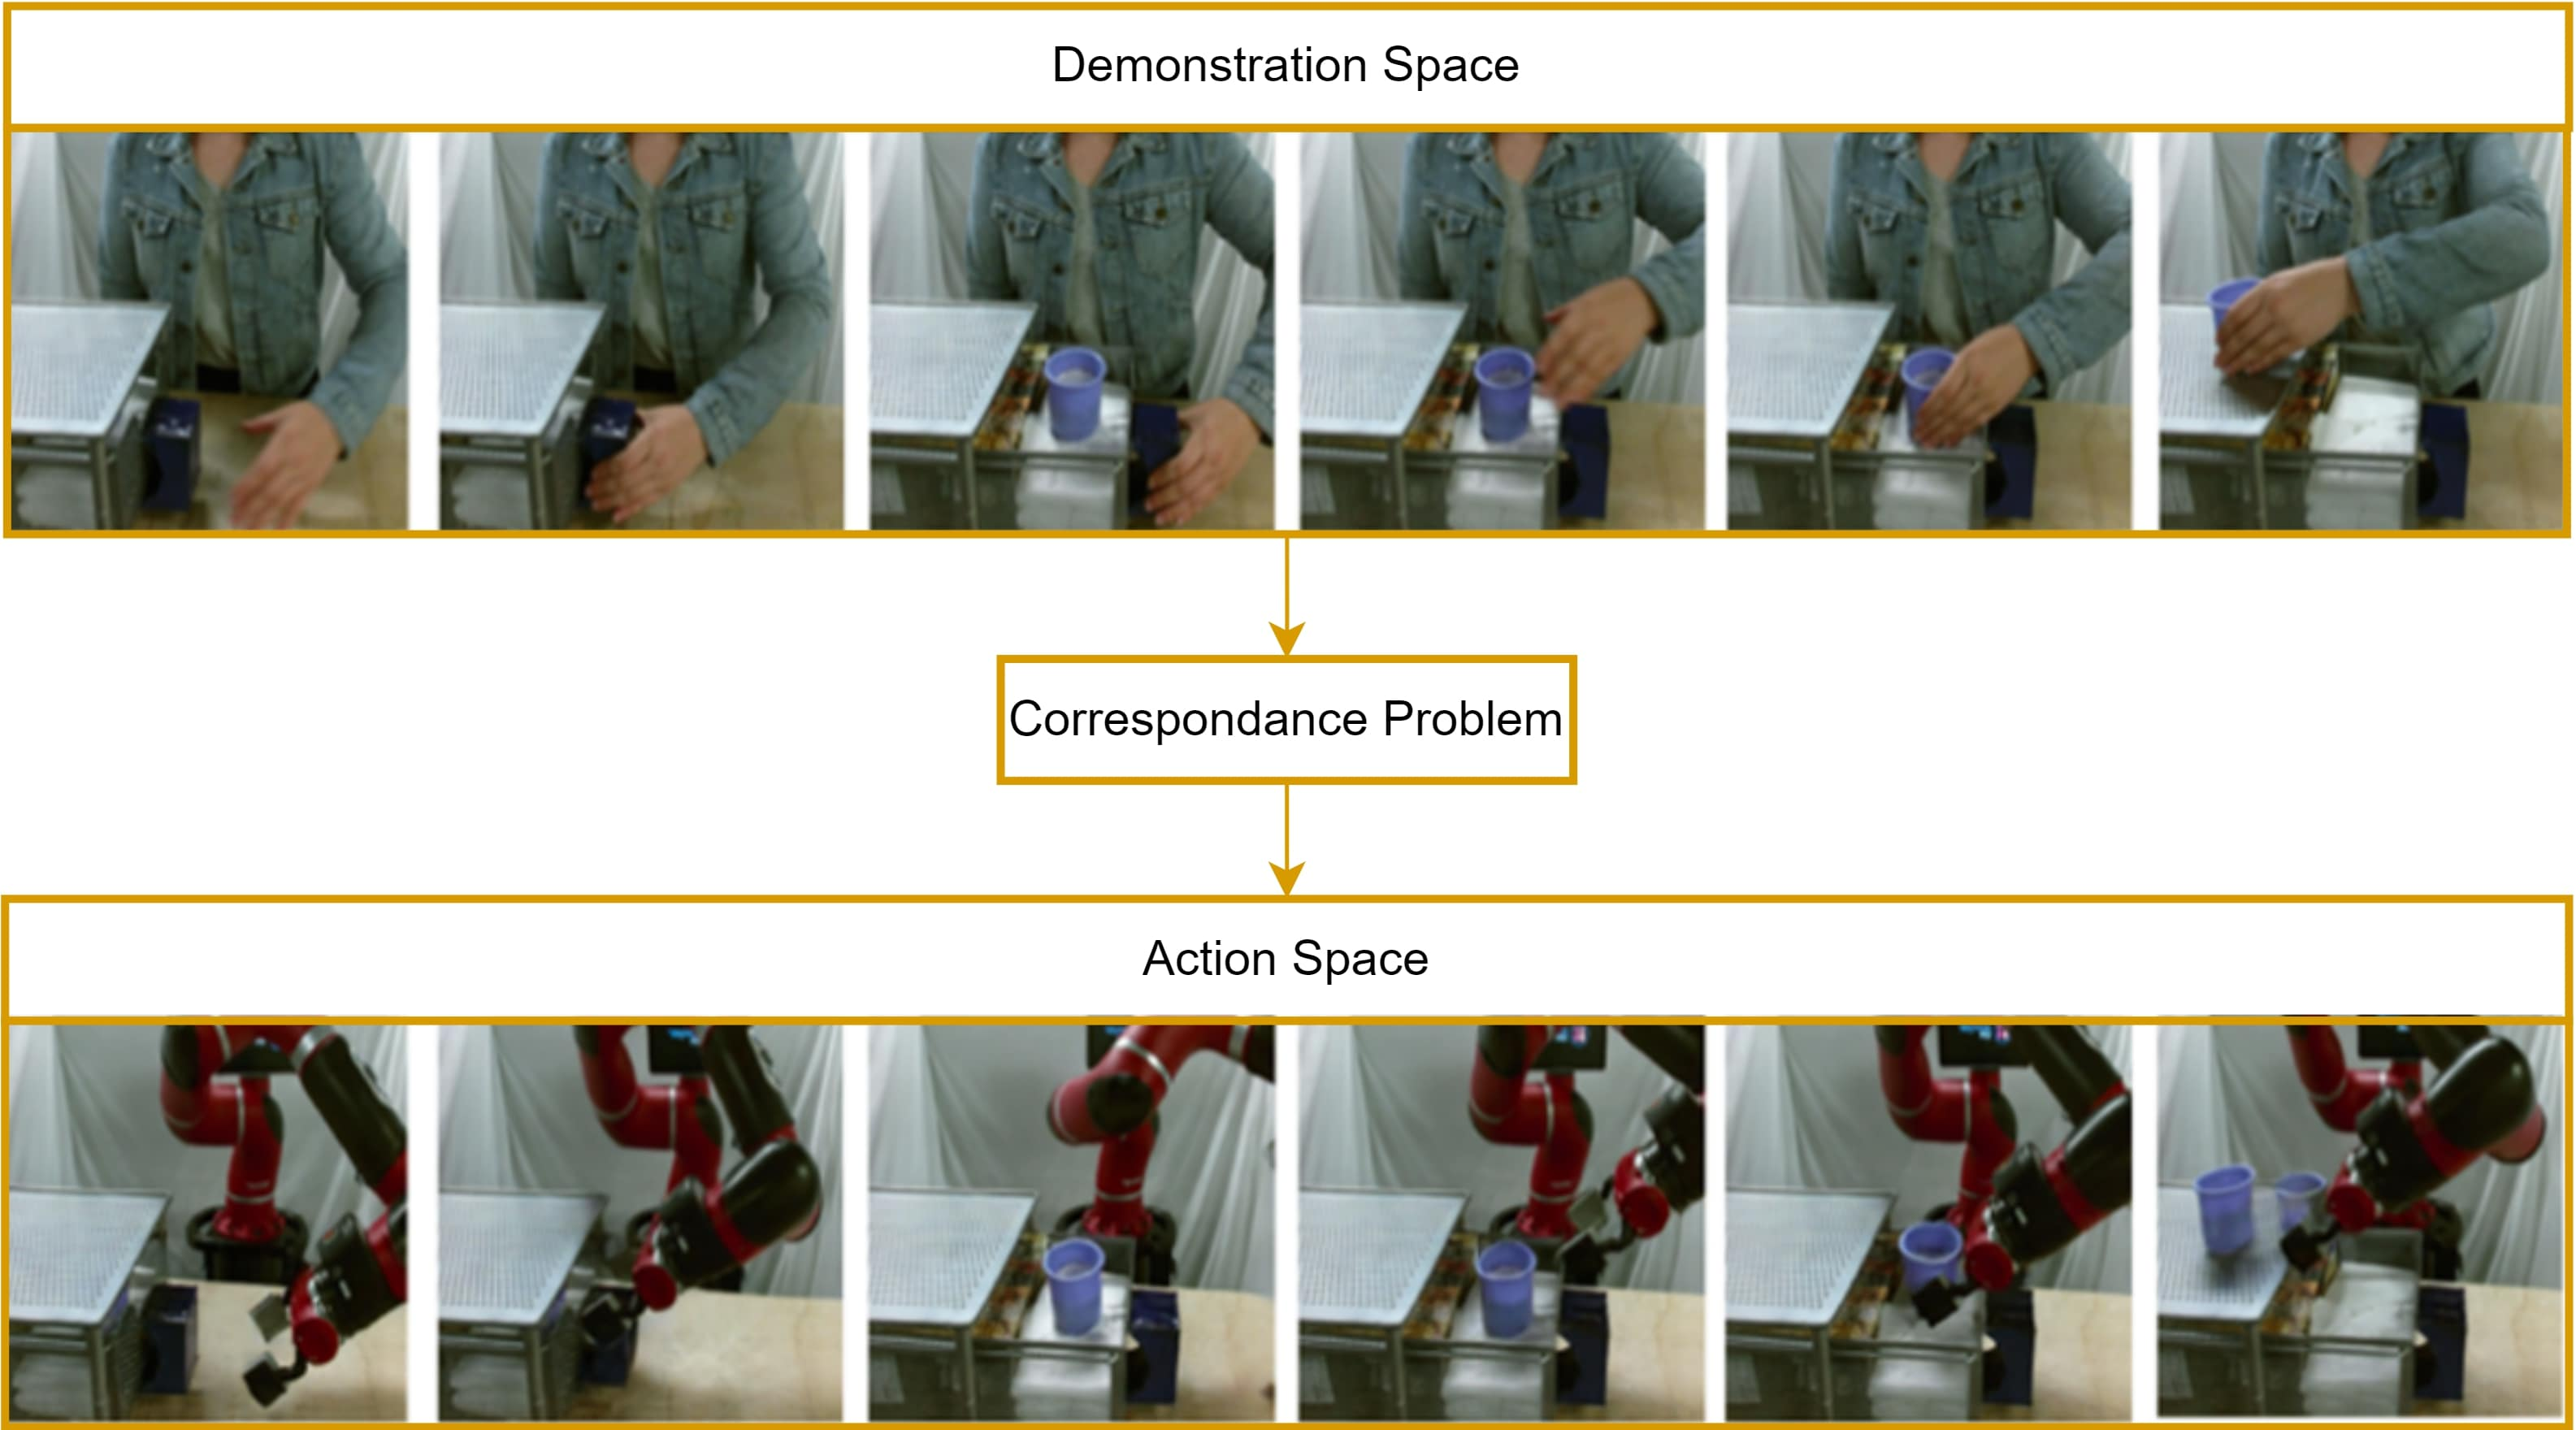
\includegraphics[width=\textwidth]{figures/images/visual_indirect_teaching.jpg}
         \caption{Example of direct demonstration based on human video demonstration~\cite{smith2019avid}.}
         \label{fig:visual_indirect}
     \end{subfigure}

    \caption{Examples of indirect demonstration.}
    \label{fig:indirect_demonstrations}
\end{figure}


\paragraph*{Indirect Demonstration}   \mbox{} \\ 
As discussed previously, in direct demonstration, an expert controls the learner agent and records the actions performed. The concept behind Indirect Demonstration (Figure \ref{fig:indirect_demonstrations}) is to collect demonstrations that are completely disconnected from the target robotic platform. In the most promising scenario, a human demonstrator performs the desired tasks and records their operations. The learner, starting from this set of recordings, must be able to extrapolate the knowledge needed to replicate the observed tasks.

In this case, the expert demonstrations are state-only trajectories. Since the action space between the human demonstrator and the robot is different (consider just the different embodiment), it is not possible to directly use the human joint trajectories to minimize a supervised loss where the predicted value is related to the robot action space.

Initially, methods that follow this approach used wearable devices to capture human movement and record it \cite{nakaoka2007learning,liu2019_mirroring_without_overimitation}. For example, in \cite{nakaoka2007learning}, the authors used a motion capture system to record the movement of a dancer and then transfer these trajectories to a humanoid robot. Similarly, in \cite{liu2019_mirroring_without_overimitation}, the authors used a tactile glove \cite{liu2017glove_force} to record the movement performed by a human hand in the operation of opening bottles (Figure \ref{fig:wearable_indirect}).

In this line of research related to indirect demonstrations, there are also novel methods \cite{smith2019avid,torabi2019recent_advances_lfo,xiong2021learning_by_watching,wang2023mimicplay,qian2024contrast} that, inspired by the way humans learn by watching task execution, remove the assumption of having access to recorded human joint trajectories. In this case, the demonstrations are just videos of the human demonstrator (Figure \ref{fig:visual_indirect}). Here, the system must infer from the video not only the intent of the task but also how this task can be solved and transform this information into its own action space.

Generally, methods based on wearable devices allow for very intuitive demonstrations, including critical information for manipulation tasks such as force and tactile information \cite{liu2019_mirroring_without_overimitation}. While methods based on just video demonstrations are very promising because they allow for the collection of demonstrations in the most intuitive and scalable way possible (potentially any video of a performed task can be used). However, both these approaches have to solve the \textit{correspondence problem}, i.e., the system must be able to map motion captured in human space into the corresponding motion of the robot. In Section \textcolor{red}{TODO}, the different ways this problem has been solved in the context of visual demonstration will be explained in detail.

